\documentclass[aspectratio=169]{beamer}

\usepackage{amsmath}
\usepackage{amssymb}
\usepackage{hyperref}
\usepackage{algorithmic}
\usepackage{graphicx}

\usepackage{booktabs}
\usepackage{subcaption}    % for subfigure environments

\theoremstyle{definition}
\usepackage[most]{tcolorbox}
\tcbset{
  definitionbox/.style={
    colback=blue!2!white,
    colframe=blue!40!black,
    title={Gaussian Random Fields Inference},
    boxrule=0.5pt,
    arc=4pt,
    top=6pt,
    bottom=6pt,
    left=6pt,
    right=6pt,
    fonttitle=\bfseries,
    enhanced,
    sharp corners,
    before skip=10pt,
    after skip=10pt
  }
}

\usepackage{tikz}
\usetikzlibrary{arrows.meta, positioning, shapes.geometric, shadows}
\usepackage[table]{xcolor}
\usepackage{booktabs}


\usepackage[style=nature, backend=biber]{biblatex}
\addbibresource{refs.bib}
\setbeamerfont{bibliography item}{size=\footnotesize}
\setbeamerfont{bibliography entry author}{size=\footnotesize}
\setbeamerfont{bibliography entry title}{size=\footnotesize}
\setbeamerfont{bibliography entry journal}{size=\footnotesize}
\setbeamerfont{bibliography entry note}{size=\footnotesize}

\newcommand\blfootnote[1]{%
  \begingroup
  \renewcommand\thefootnote{}\footnote{#1}%
  \addtocounter{footnote}{-1}%
  \endgroup
}


\title{Linear Attention: A Simple Introduction}
\author{Matthew Zhang}
\institute{Myrtle.ai}
\date{}

\begin{document}

\begin{frame}[plain]
    \titlepage
\end{frame}





\begin{frame}{Outline    \footnote{This presentation is mainly based on: Katharopoulos et al. (2020), \textit{Transformers are RNNs}.}}
    \vspace{1em}
    \begin{enumerate}
        \setlength{\itemsep}{1em}
        \item Recap: Softmax Attention
        \item Linear Attention
        \item Evolution of Linear Attention Models
        \item Code: Linear Attention v.s. Transformer
    \end{enumerate}


\end{frame}



\begin{frame}{Softmax Attention is $\mathcal{O}(T^2)$}



Let's begin with our favorite \textit{softmax attention}.

\begin{equation}
\label{eq: softmax_attn}
V^{\prime} = \text{softmax} \left( \frac{QK^T}{\sqrt{D}} \right) V
\end{equation}


where $Q, K, V \in \mathbb{R}^{T \times D}$ 


\end{frame}



\begin{frame}{Reminder: Matrix Multiplication Complexity}

For the multiplication of two matrices $A \in \mathbb{R}^{M \times N}$ and $B \in \mathbb{R}^{N \times P}$, the time complexity of computing $C = AB$ is $\mathcal{O}(M \cdot N \cdot P)$.

\begin{center}
    \renewcommand{\arraystretch}{1.5}
    \begin{tabular}{lll}
    \toprule
    \textbf{Operation} & \textbf{Shape Change} & \textbf{Complexity} \\ \midrule
    $A B$             & $(M, N) \times (N, P) \to (M, P)$ & $\mathcal{O}(M N P)$ \\
    \bottomrule
    \end{tabular}
    \end{center}

\begin{itemize}
    \item Each of the $M \times P$ elements in the resulting matrix requires $N$ scalar multiplications and additions.
\end{itemize}

\end{frame}



\begin{frame}{Softmax Attention is $\mathcal{O}(T^2)$}

\begin{equation}
V^{\prime} = \text{softmax} \left( \frac{QK^T}{\sqrt{D}} \right) V \tag{\ref{eq: softmax_attn}}
\end{equation}


where $Q, K, V \in \mathbb{R}^{T \times D}$ 

\begin{itemize}
    
    \item \textbf{Training  complexity}
    \begin{center}
    \renewcommand{\arraystretch}{1.5}
    \begin{tabular}{lll}
    \toprule
    \textbf{Operation} & \textbf{Shape Change} & \textbf{Complexity} \\ \midrule
    $QK^T$             & $(T, D) \times (D, T) \to (T, T)$ & $\mathcal{O}(T^2 D)$ \\
    $\text{softmax}(\cdot)$ & $(T, T) \to (T, T)$               & $\mathcal{O}(T^2)$    \\
    $(\cdot)V$         & $(T, T) \times (T, D) \to (T, D)$ & $\mathcal{O}(T^2 D)$ \\ \bottomrule
    \end{tabular}
    \end{center}

    \item   \textbf{Non associativity} With softmax, we cannot swap the order of matrix multiplication, i.e., 
    \[ \text{softmax}(QK^T)V \neq Q(K^T V) \]
\end{itemize}
  

\end{frame}





\begin{frame}{What if? Restoring Associativity}

\begin{itemize}
    \item \textbf{The hypothesis:} If we can decompose $\text{softmax}(QK^T)$ into $\Phi(Q)\Phi(K)^T$, for $\Phi(Q) \in \mathbb{R}^{T \times D^\prime}$, we can leverage the \textbf{associative property} of matrix multiplication.
\end{itemize}

\begin{equation}
V^{\prime} = \underbrace{\Phi(Q)}_{\in \mathbb{R}^{T \times D^{\prime}}} \left( \underbrace{\Phi(K)^T}_{\in \mathbb{R}^{D^{\prime} \times T}} \underbrace{V}_{\in \mathbb{R}^{T \times D}} \right)
\end{equation}

\begin{itemize}
    \item \textbf{New training complexity:}
    \begin{center}
    \renewcommand{\arraystretch}{1.5}
    \begin{tabular}{lll}
    \toprule
    \textbf{Operation} & \textbf{Shape Change} & \textbf{Complexity} \\ \midrule
    $\Phi(K)^T V$      & $(D', T) \times (T, D) \to (D', D)$ & $\mathcal{O}(T D D')$ \\
    $\Phi(Q) (\cdot)$  & $(T, D') \times (D', D) \to (T, D)$ & $\mathcal{O}(T D D')$ \\ \bottomrule
    \end{tabular}
    \end{center}
\end{itemize}

\end{frame}




\begin{frame}{Let's Derive Linear Attention}



Start with the softmax attention in Equation \ref{eq: softmax_attn}. Consider the $i$-th query, and unpack the softmax:

\begin{equation}
    V_i^{\prime} = \frac{\sum_{j=1}^T \operatorname{sim}(Q_i, K_j) V_j}{\sum_{j=1}^T \operatorname{sim}(Q_i, K_j)}
\end{equation}

where $\operatorname{sim}(Q_i, K_j) = \exp \left( \frac{Q_i K_j^\top}{\sqrt{d_k}} \right)$ is called a \textit{kernel} function that measure the similarity between two inputs $Q_i$ and $K_j$.

\vspace{2em}

\textcolor{red}{Question: Can we find a feature map $\phi(\cdot)$ such that $\operatorname{sim}(Q_i, K_j) = \phi(Q_i) \phi(K_j)$ ?}


\end{frame}





\begin{frame}{Let's Derive Linear Attention}

By substituting the linearized similarity $\operatorname{sim}(Q_i, K_j) = \phi(Q_i) \phi(K_j)^\top$ into the attention formula:
\begin{equation}
    V'_i = \frac{\sum_{j=1}^{T} \left( \textcolor{blue}{\phi(Q_i)} \phi(K_j)^\top \right) V_j}{\sum_{j=1}^{T} \textcolor{blue}{\phi(Q_i)} \phi(K_j)^\top}
\end{equation}

Since $\textcolor{blue}{\phi(Q_i)}$ is constant with respect to the summation index $j$, we apply the distributive property to move it outside the sum:
\begin{equation}
\label{eq: linear_attn_partial}
    V'_i = \frac{\textcolor{blue}{\phi(Q_i)} \left( \sum_{j=1}^{T} \phi(K_j)^\top V_j \right)}{\textcolor{blue}{\phi(Q_i)} \left( \sum_{j=1}^{T} \phi(K_j)^\top \right)}
\end{equation}

This factorization allows the terms in parentheses to be computed first and avoid the $\mathcal{O}(T^2)$ complexity!


\end{frame}





\begin{frame}{Let's Derive Linear Attention: Matrix Form}

To compute attention for all queries simultaneously, we define:
\begin{itemize}
    \item $\Phi(Q) \in \mathbb{R}^{T \times D'}$
    \item $\Phi(K) \in \mathbb{R}^{T \times D'}$
    \item $V \in \mathbb{R}^{T \times D}$
    \item $\mathbf{1} \in \mathbb{R}^{T \times 1}$ (vector of ones)
\end{itemize}

This simplifies Equation \ref{eq: linear_attn_partial} to 


\begin{equation}
    V'_i = \frac{\textcolor{blue}{\phi(Q_i)}   (\Phi(K)^\top V) }{\textcolor{blue}{\phi(Q_i)} \Phi(K)^\top \mathbf{1}}
\end{equation}


The full linearized attention for the entire sequence is:
\begin{equation}
    V' = \frac{\Phi(Q) \left( \Phi(K)^\top V \right)}{\Phi(Q) \left( \Phi(K)^\top \mathbf{1} \right)}
\end{equation}
\textit{Note: The division is performed row-wise.}

\end{frame}




\begin{frame}{Let's Derive Linear Attention: Training Complexity}

\begin{center}
\renewcommand{\arraystretch}{1.2}
\begin{tabular}{@{}lll@{}}
\toprule
\textbf{Operation} & \textbf{Shape Change} & \textbf{Complexity} \\ \midrule
\rowcolor{gray!10} \multicolumn{3}{l}{\textit{Numerator: $\Phi(Q) (\Phi(K)^\top V)$}} \\
$\Phi(K)^\top V$      & $(D', T) \times (T, D) \to (D', D)$ & $\mathcal{O}(T D D')$ \\
$\Phi(Q) (\cdot)$     & $(T, D') \times (D', D) \to (T, D)$ & $\mathcal{O}(T D D')$ \\ \addlinespace

\rowcolor{gray!10} \multicolumn{3}{l}{\textit{Denominator: $\Phi(Q) (\Phi(K)^\top \mathbf{1})$}} \\
$\Phi(K)^\top \mathbf{1}$ & $(D', T) \times (T, 1) \to (D', 1)$ & $\mathcal{O}(T D')$ \\
$\Phi(Q) (\cdot)$         & $(T, D') \times (D', 1) \to (T, 1)$ & $\mathcal{O}(T D')$ \\ \addlinespace

\rowcolor{gray!10} \multicolumn{3}{l}{\textit{Normalization}} \\
Row-wise Division & $(T, D) \text{ by } (T, 1)$ & $\mathcal{O}(T D)$ \\ \bottomrule
\end{tabular}
\end{center}

\vspace{0.5em}
\begin{itemize}
    \item The total training complexity is dominated by $\mathcal{O}(T D D')$.
    \item \textbf{Result:} We have successfully replaced $\mathcal{O}(T^2)$ with linear $\mathcal{O}(T)$.
\end{itemize}
    
\end{frame}






\begin{frame}{Deriving the Feature Map: 1st Order Approx}

To linearize attention, we seek a feature map $\phi(\cdot)$ such that $\operatorname{sim}(Q_i, K_j) \approx \phi(Q_i)\phi(K_j)^\top$. 

\vspace{0.5em}
Consider the first-order Taylor expansion of the exponential (ignoring the $\sqrt{d_k}$ scaling):
\begin{equation}
    \exp(Q_i K_j^\top) \approx 1 + Q_i K_j^\top
\end{equation}

For row vectors $Q_i, K_j \in \mathbb{R}^{1 \times d}$, we define the feature map:
\begin{equation}
    \phi(x) = \begin{bmatrix} 1 & x \end{bmatrix} \in \mathbb{R}^{1 \times (1+d)}
\end{equation}

Then the inner product $\phi(Q_i)\phi(K_j)^\top$ is:
\begin{equation}
    \begin{bmatrix} 1 & Q_i \end{bmatrix} \begin{bmatrix} 1 \\ K_j^\top \end{bmatrix} = 1 + Q_i K_j^\top
\end{equation}

This shows that a simple concatenation of a bias term and the raw input recovers the first-order approximation of the exponential kernel.

\end{frame}

\begin{frame}{Deriving the Feature Map: Full Exponential Kernel}

To recover the exact softmax attention, we expand the exponential to its full Taylor series:
\begin{equation}
    \exp(Q_i K_j^\top) = \sum_{n=0}^{\infty} \frac{(Q_i K_j^\top)^n}{n!} = 1 + Q_i K_j^\top + \frac{(Q_i K_j^\top)^2}{2!} + \dots
\end{equation}

This corresponds to an \textbf{infinite-dimensional} feature map $\phi(x)$. To ensure the inner product $\phi(Q_i)\phi(K_j)^\top$ distributes the $1/n!$ correctly, we define:
\begin{equation}
    \phi(x) = \left[ 1, x, \frac{x^{\otimes 2}}{\sqrt{2!}}, \dots, \frac{x^{\otimes n}}{\sqrt{n!}}, \dots \right]
\end{equation}
where $x^{\otimes n}$ is the $n$-th order self-tensor product. 


\end{frame}


\begin{frame}{What is the $\phi(\cdot)$ used in literature?}

In practice, any feature map $\phi: \mathbb{R}^D \to \mathbb{R}^{D'}$ defines a valid \textit{kernel} if it satisfies the \textbf{positivity constraint}:
\begin{equation}
    \phi(x) \geq 0 \quad (\text{element-wise})
\end{equation}
This ensures numerical stability and prevents a zero or negative denominator.

\vspace{1em}

\begin{center}
\renewcommand{\arraystretch}{1.4}
\begin{tabular}{lll}
\toprule
\textbf{Model} & \textbf{Feature Map } $\phi(x)$ & \textbf{Goal} \\ \midrule
\textbf{Linear Transformer} & $\text{elu}(x) + 1$ & Efficiency/Simplicity \\
\textbf{Performer} & Random Fourier Features & Softmax Approx. \\
\textbf{Mamba-2 (SSD)} & Implicit (State Expansion) &  \\ \bottomrule
\end{tabular}
\end{center}



\end{frame}





\begin{frame}{Causal Masking in Linear Attention}
To train autoregressive models, position $i$ must only be influenced by positions $j \leq i$. The linearized formulation becomes:
\begin{equation}
    V'_i = \frac{\phi(Q_i)^T \sum_{j=1}^i \phi(K_j) V_j^T}{\phi(Q_i)^T \sum_{j=1}^i \phi(K_j)}
\end{equation}

By defining the cumulative states $S_i$ and $Z_i$:
\begin{equation}
    S_i = \sum_{j=1}^i \phi(K_j) V_j^T, \quad Z_i = \sum_{j=1}^i \phi(K_j)
\end{equation}

The output is simplified to:
\begin{equation}
    V'_i = \frac{\phi(Q_i)^T S_i}{\phi(Q_i)^T Z_i}
\end{equation}
\textit{Note: $S_i$ and $Z_i$ can be updated from $S_{i-1}$ and $Z_{i-1}$ in constant time.}
\end{frame}


\begin{frame}{Make Inference Like an RNN}
Causal linear attention layers can be viewed as RNNs where $S_i$ and $Z_i$ act as internal hidden states (memory).

\textbf{State Updates:}
\begin{align}
    s_i &= s_{i-1} + \phi(x_i W_K) (x_i W_V)^T \\
    z_i &= z_{i-1} + \phi(x_i W_K)
\end{align}

\textbf{Output Prediction:}
\begin{equation}
    y_i = f_l \left( \frac{\phi(x_i W_Q)^T s_i}{\phi(x_i W_Q)^T z_i} + x_i \right)
\end{equation}

\begin{itemize}
    \item $s_i$: Attention memory (feature-value interactions)
    \item $z_i$: Normalizer memory (cumulative features)
    \item $f_l$: feed-forward + RMSNorm 
    \item $x_i$: residual connection.
\end{itemize}
\end{frame}



\begin{frame}{Linear Attention: Summary}

\begin{equation}
\text{Attention}(Q, K, V) = \frac{\Phi(Q) \left( \Phi(K)^\top V \right)}{\Phi(Q) \left( \Phi(K)^\top \mathbf{1} \right)}
\end{equation}

\vspace{0.5em}

\begin{itemize}
    \item $\Phi(Q), \Phi(K) \in \mathbb{R}^{T \times D}, \quad V \in \mathbb{R}^{T \times D}$

    \vspace{0.5em}
    
    \item Training complexity: $\mathcal{O}(T)$ :

    \vspace{0.5em}
    \item Inference complexity: $\mathcal{O}(1)$
    \begin{enumerate}
        \item Update KV State: $S_{new} = S_{old} + k_{new}^T v_{new} \hfill \mathcal{O}(D^2)$
        \item Update Normalizer: $z_{new} = z_{old} + k_{new} \hfill \mathcal{O}(D)$
        \item Compute Output: $y_{new} = f_l \left( \frac{q_{new} S_{new}}{q_{new} z_{new}^T} + x_{new} \right) \hfill \mathcal{O}(D^2)$
    \end{enumerate}
\end{itemize}

\end{frame}




\begin{frame}{(Simplified) Evolution of Linear Attention \& SSMs}
\centering

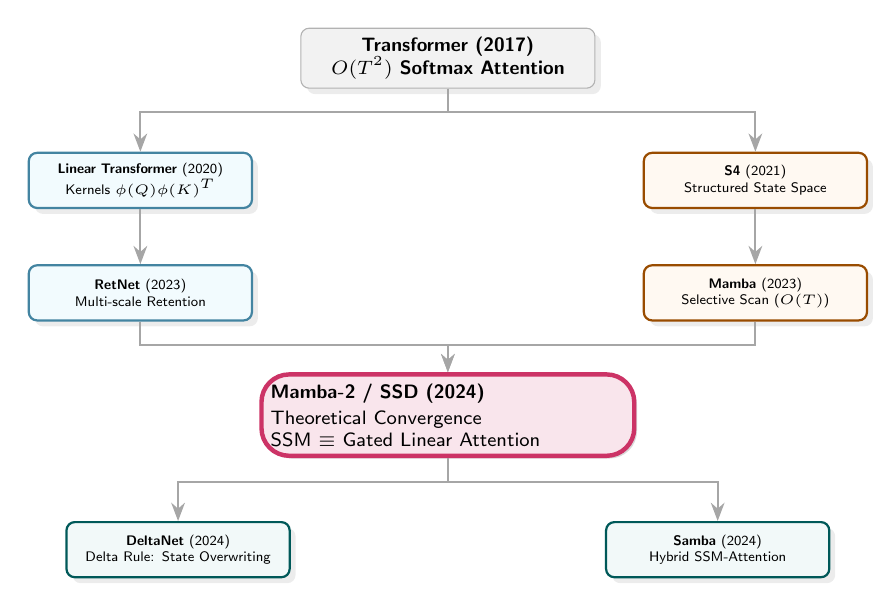
\begin{tikzpicture}[
    node distance=0.8cm and 0.5cm,
    base/.style={rectangle, draw, rounded corners=3pt, font=\sffamily\tiny, align=center, minimum height=0.7cm, text width=2.6cm, drop shadow={opacity=0.15}, fill=white},
    root/.style={base, fill=gray!10, draw=gray!60, text width=3.5cm, font=\sffamily\bfseries\scriptsize},
    ssm/.style={base, fill=orange!5, draw=orange!60!black, thick},
    lin/.style={base, fill=cyan!5, draw=cyan!60!black, thick},
    % Convergence Node - Bolding only the first line
    conv/.style={draw=purple!80, fill=purple!10, ultra thick, rounded corners=10pt, font=\sffamily\scriptsize, text width=4.5cm, drop shadow={opacity=0.3, shadow xshift=1pt, shadow yshift=-1pt}},
    modern/.style={base, fill=teal!5, draw=teal!70!black, thick},
    arrow/.style={-{Stealth[scale=1.0]}, thick, draw=gray!70}
]

    % --- Nodes ---
    \node[root] (trans) {Transformer (2017) \\ $O(T^2)$ Softmax Attention};

    % Linear Branch
    \node[lin, below left=0.8cm and 0.6cm of trans] (linattn) {\textbf{Linear Transformer} (2020) \\ Kernels $\phi(Q)\phi(K)^T$};
    \node[lin, below=0.7cm of linattn] (retnet) {\textbf{RetNet} (2023) \\ Multi-scale Retention};

    % SSM Branch
    \node[ssm, below right=0.8cm and 0.6cm of trans] (s4) {\textbf{S4} (2021) \\ Structured State Space};
    \node[ssm, below=0.7cm of s4] (mamba) {\textbf{Mamba} (2023) \\ Selective Scan ($O(T)$)};

    % Convergence (Mamba-2) - Selective Bolding
    \node[conv, below=3.6cm of trans] (mamba2) {{\textbf{Mamba-2 / SSD (2024)}} \\[0.2em] Theoretical Convergence \\ SSM $\equiv$ Gated Linear Attention};

    % Post-Convergence
    \node[modern, below left=0.8cm and -0.4cm of mamba2] (deltanet) {\textbf{DeltaNet} (2024) \\ Delta Rule: State Overwriting};
    \node[modern, below right=0.8cm and -0.4cm of mamba2] (samba) {\textbf{Samba} (2024) \\ Hybrid SSM-Attention};

    % --- Connections ---
    \draw[arrow] (trans.south) -- ++(0,-0.3) -| (linattn.north);
    \draw[arrow] (trans.south) -- ++(0,-0.3) -| (s4.north);
    
    \draw[arrow] (linattn.south) -- (retnet.north);
    \draw[arrow] (s4.south) -- (mamba.north);
    
    \draw[arrow] (retnet.south) -- ++(0,-0.3) -| (mamba2.north);
    \draw[arrow] (mamba.south) -- ++(0,-0.3) -| (mamba2.north);
    
    \draw[arrow] (mamba2.south) -- ++(0,-0.3) -| (deltanet.north);
    \draw[arrow] (mamba2.south) -- ++(0,-0.3) -| (samba.north);

\end{tikzpicture}

\end{frame}






\begin{frame}{My Coding Demo: Linear Models vs. Llama}

    \vspace{1cm}
    \centering
    \textbf{Demo Repository:} \\

      \vspace{1cm}
    
    \url{https://github.com/MatthewZhang473/linear-attention-demo}

\end{frame}



\begin{frame}{What we are NOT covering today (but I also find interesting) }

\begin{itemize}
    \item Hardware (GPU) efficient algorithms, e.g. block-matrix decomposition

    \item (Unfortunately) the model architectures
\end{itemize}
    
\end{frame}


\begin{frame}{Next: State Space Models}

\begin{figure}
    \centering
    \includegraphics[width=1.0\linewidth]{images/Mamba.png}
    \label{fig:Mamba1}
\end{figure}
    
\end{frame}



\begin{frame}[allowframebreaks]{References}
    \nocite{*} 
    \printbibliography
\end{frame}


\end{document}